\section{Global-view Communication and Synchronization Constructs}

\subsection{{\tt reflect} Construct}

\subsubsection*{Synopsis}

The {\tt \Directive{reflect}} construct assigns the value of a
reflection source to the corresponding shadow object for variables
having the shadow attribute. 

\subsubsection*{Syntax}
\Syntax{reflect}

\begin{tabular}{ll}
 \verb![F]! & \verb|!$xmp| {\tt reflect} \verb|(| {\it array-name}
 {\openb}, {\it array-name}{\closeb}... \verb|)|\\
 &\hspace{3cm} {\openb}{\tt width (} {\it reflect-width} {\openb}, {\it
     reflect-width}{\closeb}... {\tt )}{\closeb}
     {\openb}{\tt async (} {\it async-id} {\tt )}{\closeb} \\
\verb![C]! & \verb|#pragma xmp| {\tt reflect} \verb|(| {\it array-name}
     {\openb}, {\it array-name}{\closeb}... \verb|)|\\
 &\hspace{3cm} {\openb}{\tt width (} {\it reflect-width} {\openb}, {\it
     reflect-width}{\closeb}... {\tt )}{\closeb}
     {\openb}{\tt async (} {\it async-id} {\tt )}{\closeb} \\
\end{tabular}

\vspace{0.3cm}

where {\it reflect-width} must be one of:

\vspace{0.3cm}

\begin{tabular}{ll}
 \hspace{0.5cm} & {\openb}{\tt /periodic/}{\closeb} {\it int-expr} \\
                & {\openb}{\tt /periodic/}{\closeb} {\it int-expr} : {\it int-expr}
\end{tabular}

\subsubsection*{Description}

The {\tt reflect} construct updates each of the shadow object of the
array specified by {\it array-name} with the value of its corresponding
reflection source. Note that the shadow objects for
``obliquely-neighboring'' elements can be also updated with this
construct.

%copies the value of the reflection source of
%the reflect-object specified by {\it array-name} to all shadow
%objects.
%This directive may execute the communications.

When the {\tt width} clause is specified and of the form ``{\it
int-expr} : {\it int-expr},'' the shadow area of the width specified by
the first {\it int-expr} at the upper bound and that specified by the
second one at the lower bound in the specified dimension are updated.
%
When the {\tt width} clause is specified and of the form {\it int-expr},
the shadow areas of the same width specified at both the upper
and lower bounds in the specified dimension are updated.
%
When the {\tt width} clause is omitted, whole shadow area of the array
is updated.

Particularly when the {\tt /periodic/} modifier is specified in {\it
reflect-width}, the update of the shadow object in the dimension is
``periodic,'' which means that the shadow object at the global lower
(upper) bound is treated as if corresponding to the data object of the
global upper (lower) bound and updated with that value in the {\tt
reflect} construct.

When the {\tt async} clause is specified, the statements following this
construct may be executed before the operation is complete.

\subsubsection*{Restrictions}

\begin{itemize}
 \item The arrays specified by the sequence of {\it array-name} must be
       mapped onto the executing node set.
 \item The reflect width of each dimension specified by {\it
       reflect-width} must not exceed the shadow width of the arrays.
 \item The {\tt reflect} construct is global, which means that it must be
       executed by all of the executing nodes, and each local variable
       referenced in the construct must have the same value among all of
       them.
 \item {\it async-id} must be an expression of type default integer, in
       Fortran, or type {\tt int}, in C.
\end{itemize}

\subsubsection*{Example}
\Example{reflect}
\Example{shadow}

\begin{Fexample}
!$xmp nodes p(4)
!$xmp template t(100)
!$xmp distribute t(block) onto p:: t

      real a(100)
!$xmp align a(i) with t(i)
!$xmp shdow a(1)

      ...
!$xmp reflect (a) width (/periodic/1)
\end{Fexample}

\begin{myfigure}
\begin{center}
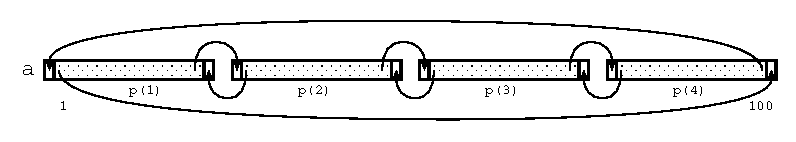
\includegraphics[width=0.7\hsize]{figs/fig3.2.eps}
\end{center}
\caption{Example of Periodic Shadow Reflection}
\label{fig3.2}
\end{myfigure}

The {\tt shadow} directive allocates ``periodic'' shadow areas 
The {\tt reflect} construct updates ``periodically'' the shadow area of
the array {\tt a} (Figure \ref{fig3.2}). A periodic shadow at the lower
bound on the node {\tt p(1)} is updated with the value of {\tt a(100)}
and that at the upper bound on {\tt p(4)} with the value of {\tt a(1)}.


\subsection{{\tt gmove} Construct}

\subsubsection*{Synopsis}

%The {\tt \Directive{gmove}} construct copies the data of a
%distributed array in the global view. 

The {\tt \Directive{gmove}} construct allows an assignment statement,
which may cause communication, to be executed possibly in parallel by
the executing nodes.

\subsubsection*{Syntax}
\Syntax{gmove}

\begin{tabular}{ll}
\verb![F]! & \verb|!$xmp| {\tt gmove} {\openb}{\tt in} $\vert$ {\tt
 out}{\closeb} {\openb}{\tt async (} {\it async-id} {\tt )}{\closeb}\\
% {\it dest} {\tt =} {\it source} \\
\verb![C]! & \verb|#pragma xmp| {\tt gmove} {\openb}{\tt in} $\vert$ {\tt
     out}{\closeb} {\openb}{\tt async (} {\it async-id} {\tt )}{\closeb}\\
% {\it dest} {\tt =} {\it source} \\
\end{tabular}

\subsubsection*{Description}

This construct copies the value of the right-hand side variable into
the left-hand side of the associated assignment statement, which may
require communication between nodes in the executing node set. Such
communication is detected, scheduled, and performed by the XcalableMP
runtime system.

%This construct executes a copy operation of the global data array object
%distributed into nodes.
%This directive is followed by the assignment
%statement of the scalar value and array sections.
%The assignment may require communication between nodes.

%Note that, in {\XMP}, the {\C} language is extended to support array
%section notation in order to support an assignment of array objects.

%The assignment statement must have one of the following patterns:
%
%\begin{itemize}
%\item  Scalar assignment. For example:
%
%\begin{tabular}{lll}
%\hspace{0.5cm} & {\tt s1 = s2} & ! {\tt s1} and {\tt s2} is a scalar
%variable \\ 
%& {\tt a(3) = b(i, j)} & ! {\tt a} and {\tt b} are arrays. \\
%\end{tabular}
%
%\item Array assignment. The left-hand-side variable must be either an
%      array name, an array section, or a scalar object. For example:
%
%\begin{tabular}{lll}
%\hspace{0.5cm} & {\tt a = b} & ! {\tt a} and {\tt b} are arrays \\
% & {\tt a(1:10) = b(n:n+9, k)} & ! lhs and rhs are array sections \\
% & {\tt a(1:10) = s2} & ! lhs is an array section and rhs is a
% scalar variable \\
% & {\tt a(1:10) = b(i, j)} & ! lhs is an array section and rhs is a
% scalar object \\
%\end{tabular}
%\end{itemize}

%The {\tt gmove} construct must be executed by all of the executing
%nodes. The value of scalar objects, the index value, and the range
%value of the array section in the assignment statement must be the same in
%every node executing this directive.

There are three operating modes of the {\tt gmove} construct:

\begin{itemize}
 \item {\bf collective mode}

       When neither the {\tt in} nor the {\tt out} clause is specified,
       the copy operation is performed collectively and cause an
       implicit synchronization after it inside the executing node set.

%In this case, all elements in both the source array and the target array
%must be distributed onto the executing node set.
%If the object on the right-hand side is a local
%object, then the value of the local object must be the same.
%
%In this case, the assignment is performed locally, where the object on
%the left-hand side is distributed.
%
%If the object on the left-hand side is a local object
%and the object on the right-hand side is global, then this operation
%performs broadcast operation.

 \item {\bf in mode}

       When the {\tt in} clause is specified, the rhs data of the
       assignment, whole or parts of which may reside outside the
       executing node set, can be transferred from its owner nodes.

       If the {\tt async} clause is not specified, then the construct is
       ''synchronous'' and it is guaranteed that the lhs data
       can be read and overwritten and all of the operations of the
       construct on the owner nodes (origin) and the executing node
       (target) are completed when returning from the construct;
       otherwise, the construct is ''asynchronous'' and it is not
       guaranteed until returning from the associating {\tt wait\_async}
       construct.

 \item {\bf out mode}

       When the {\tt out} clause is specified, the lhs data of the
       assignment, whole or parts of which may reside outside the 
       executing node set, can be transferred to its owner nodes.

       If the {\tt async} clause is not specified, then the construct is
       ''synchronous'' and it is guaranteed that the rhs data
       can be overwritten and all of the operations of the construct on
       the owner nodes (origin) and the executing node (target) are
       completed when returning from the construct; otherwise, the
       construct is ''asynchronous'' and it is not guaranteed until
       returning from the associating {\tt wait\_async} construct.

\end{itemize}

%Note that, in these cases, no synchronization is implied and it is not
%ensured that the copy operation is completed. Thus, if a synchronization
%between the executing nodes and the owner nodes is required, the
%programmer must specify it explicitly by using a {\tt barrier} construct
%or a pair of a {\tt post} and an {\tt wait} construct.

%When an {\tt in} clause is specified, then the node that owns the
%element of the object on the left-hand side obtains the data on the
%right-hand side by the remote copy (get) operation.
%Therefore, the object on the left-hand side must be distributed onto
%the executing node set.
%
%When an {\tt out} clause is specified, then the node that owns the element
%of the object on the right-hand side places the data on the left-hand
%side by the remote copy (put) operation.
%Therefore, the object on the
%right-hand side must be distributed onto the executing node set.

%If no option is specified, then the copy can be performed by two-side
%communication. In this case, the receiver side waits for the sender side,
%resulting in implicit synchronization. 

%If an {\tt in} or {\tt out} clause is specified, then the
%copy operation should be performed by one-side communication for remote
%memory access. Thus, no synchronization is implied. If
%synchronization between reader and writer is required, then the programmer
%must perform synchronization explicitly by a {\tt barrier} construct. If
%the reader and the writer do not belong to the same executing node set,
%then point-to-point synchronization by {\tt post-wait} directive can be used.

When the {\tt async} clause is specified, the statements following this
construct may be executed before the operation is complete.

\subsubsection*{Restrictions}

\begin{itemize}
 \item The {\tt gmove} directive must be followed by (i.e. associated
       with) a simple assignment statement that contains neither
       arithmetic operations nor function calls.
 \item The {\tt gmove} construct is global, which means that it must be
       executed by all of the executing nodes, and each local variable
       referenced in the construct must have the same value among all of
       them.
 \item If the {\tt gmove} construct is in {\it collective} mode, then
       all elements of the distributed arrays appearing in both the
       left-hand and the right-hand side of the associated assignment
       statement must reside in the executing node set.
 \item If the {\tt gmove} construct is in {\it in} mode, then
       all elements of the distributed array appearing in the left-hand
       side of the associated assignment statement must reside in the
       executing node set.
 \item If the {\tt gmove} construct is in {\it out} mode, then
       all elements of the distributed array appearing in the right-hand
       side of the associated assignment statement must reside in the
       executing node set.
 \item {\it async-id} must be an expression of type default integer, in
       Fortran, or type {\tt int}, in C.
\end{itemize}

\subsubsection*{Examples}
\begin{description}
\item[Example 1: Array assignment]
\Example{gmove}

If both the left-hand side and the right-hand side are distributed
arrays, then the copy operation can be performed by all-to-all
communication. If the left-hand side is a replicated array, this copy
is performed by multi-cast communication. If the right-hand side is a
replicated array, then no communication is required.

\vspace{0.5cm}

\begin{minipage}{0.45\hsize}
\begin{center}
\begin{Fexample}
!$xmp gmove
      a(:,1:N) = b(:,3,0:N-1)
\end{Fexample}
\end{center}
\end{minipage}
\begin{minipage}{0.45\hsize}
\begin{center}
\begin{CexampleR}
#pragma xmp gmove
      a[1:N][:] = b[0:N-1][3][:];
\end{CexampleR}
\end{center}
\end{minipage}
\vspace{1cm}

\item[Example 2: Scalar assignment to an array] 

When the right-hand side is an element of a distributed array, the copy
is performed by broadcast communication from the owner of the element. If 
the right-hand side is a replicated array, then no communication is required.

\vspace{0.5cm}

\begin{minipage}{0.45\hsize}
\begin{center}
\begin{Fexample}
!$xmp gmove
      a(:,1:N) = c(k)
\end{Fexample}
\end{center}
\end{minipage}
\begin{minipage}{0.45\hsize}
\begin{center}
\begin{CexampleR}
#pragma xmp gmove
      a[1:N][:] = c[k]
\end{CexampleR}
\end{center}
\end{minipage}
\vspace{1cm}

\item[Example 3: in mode assignment]

	   Since {\tt b(3)} referenced in the right-hand side of the
	   {\tt gmove} construct does not reside in the executing node
	   set ({\tt p(1:2)}), the construct is executed in in
	   mode. Thus, {\tt b(3)} is transferred from its owner node
	   {\tt p(3)} to the executing node set.

	   It is not guaranteed until {\tt p(1:2)} returns from the
	   construct that any node can read and overwrite {\tt a(1:2)}
	   and any relevant operations on {\tt p(1:2)} and {\tt p(3)}
	   are completed.

\vspace{0.5cm}

\begin{Fexample}
!$xmp nodes p(4)
!$xmp template t(4)
!$xmp distribute t(block) onto p

      real a(4), b(4)
!$xmp align (i) with t(i) : a, b
      ...
!$xmp task on p(1:2)
      ...
!$xmp gmove in
      a(1:2) = b(2:3)
      ...
!$xmp end task
\end{Fexample}

%$

\end{description}

\subsection{{\tt barrier} Construct}

\subsubsection*{Synopsis}

The {\tt \Directive{barrier}} construct specifies an explicit barrier
at the point at which the construct appears. 

\subsubsection*{Syntax}
\Syntax{barrier}

\begin{tabular}{ll}
\verb![F]! & \verb|!$xmp| {\tt barrier} {\openb}{\tt on} {\it nodes-ref}
 $\vert${\it template-ref}{\closeb} \\
\verb![C]! & \verb|#pragma xmp| {\tt barrier} {\openb}{\tt on} {\it
     nodes-ref} $\vert$ {\it template-ref}{\closeb} \\
\end{tabular}

\subsubsection*{Description}

The barrier operation is performed among the node set specified by
the {\tt on} clause. If no {\tt on} clause is specified, then it is
assumed that the current executing node set is specified in it.

Note that an {\tt on} clause may represent multiple node sets. In such a
case, a barrier operation is performed in each node set.

%The barrier construct also has the function of ensuring that all of the
%remote copy operations that are invoked by gmove in/out constructs
%executed by the node set specified by the {\tt on} clause are finished.

\subsubsection*{Restriction}

\begin{itemize}
\item The node set specified by the {\tt on} clause must be a subset of the
      executing node set.  
\end{itemize}


\subsection{{\tt reduction} Construct}

\subsubsection*{Synopsis}

The {\tt \Directive{reduction}} construct performs a reduction
operation among nodes. 

\subsubsection*{Syntax}
\Syntax{reduction}

\begin{tabular}{ll}
\verb![F]! & \verb|!$xmp| {\tt reduction (} {\it reduction-kind} {\it
  :} {\it variable} {\openb}, {\it variable} {\closeb}... {\tt )}\\
 & \hspace{6cm} {\openb}{\tt on} {\it node-ref} $\vert$ {\it
     template-ref}{\closeb} {\openb}{\tt async (} {\it async-id} {\tt
     )}{\closeb} \\
\end{tabular}

\vspace{0.5cm}

where {\it reduction-kind} is one of:

\begin{tabular}{ll}
 \hspace{0.5cm} & {\tt +} \\
 & {\tt *} \\
 & {\tt -} \\
 & {\tt .AND.} \\
 & {\tt .OR.} \\
 & {\tt .EQV.} \\
 & {\tt .NEQV.} \\
 & {\tt MAX} \\
 & {\tt MIN} \\
 & {\tt IAND} \\
 & {\tt IOR} \\
 & {\tt IEOR} \\
\end{tabular}

\vspace{0.5cm}

\begin{tabular}{ll}
 \hspace{-\parindent}
 \verb![C]! & \verb|#pragma xmp| {\tt reduction (} {\it reduction-kind} {\it
  :} {\it variable} {\openb}, {\it variable} {\closeb}... {\tt )}\\
 & \hspace{6cm} {\openb}{\tt on} {\it node-ref} $\vert$ {\it
     template-ref}{\closeb} {\openb}{\tt async (} {\it async-id} {\tt
     )}{\closeb} \\
\end{tabular}

\vspace{0.5cm}

where {\it reduction-kind} is one of:

\begin{tabular}{ll}
 \hspace{0.5cm} & {\tt +} \\
 & {\tt *} \\
 & {\tt -} \\
 & {\verb|&|} \\
 & {\tt |} \\
 & {\verb|^|} \\
 & {\verb|&&|} \\
 & {\tt ||} \\
 & {\tt max} \\
 & {\tt min} \\
\end{tabular}

\subsubsection*{Description}

The {\tt reduction} construct performs a type of
% modified by Sakagami,H. 09/11/13                                            
reduction operation specified by {\it reduction-kind} for the specified
local variables among the node set specified by the {\tt on}
clause and sets the reduction results to the variables in each
node.
%
Note that some of the reduction operation ({\tt FIRSTMAX}, {\tt
FIRSTMIN}, {\tt LASTMAX}, and {\tt LASTMIN}) that could be specified in
the {\tt reduction} clause of the {\tt loop} directive cannot be
specified in the {\tt reduction} construct, because their semantics are
not defined in it.
%
The variable specified by {\it variable}, which is the target of the
reduction operation, is referred to as the ``\Term{reduction
variable}''. Thus, after the reduction operation, the value of the
reduction variable becomes the same in every node that performs the
operatoin.

The reduction result is computed by combining the reduction variables on
all of the nodes using the reduction operator. The ordering of this
reduction is implementation-dependent.

When the {\tt async} clause is specified, the statements following this
construct may be executed before the operation is complete.

% inserted by Sakagami,H. 09/11/13 ----- start ----                            
When {\it template-ref} is specified in the {\tt on} clause, the operation
is performed in a node set that consists of nodes onto which the
specified subset of the template is distributed.
Therefore, before the {\tt reduction} construct is executed, the
referenced template must be fixed.
%
%When {\it template-subscript} in the {\it template-ref} is ``*'', nodes
%in the corresponding dimension are ignored for the reduction operation.
%
%When {\it template-subscript} in the {\it template-ref} is {\it
%triplet}, nodes for all template elements in the corresponding dimension
%perform the reduction operation.

When {\it nodes-ref} is specified in the {\tt on} clause, the operation
is performed in the specified node set.
%Therefore, before the {\tt \Directive{reduction}} construct is executed,
%the referenced node set must be fixed.

When the {\tt on} clause is omitted, the operation is performed in the
executing node set.

Note that an {\tt on} clause may represent multiple node sets. In such a
case, a barrier operation is performed in each node set.

\subsubsection*{Restrictions}

\begin{itemize}
%\item {\it template-spec} appearing in {\it template-ref} must be either ``*'', ``\
%:'' or the range.
%\item If {\tt on} clause is omitted, the operation is done in the current execu\
%ting node.
 \item The variables specified by the sequence of {\it variable} must
       either not be aligned or be replicated among nodes of the node
       set specified by the {\tt on} clause.
 \item The {\tt reduction} construct is global, which means that it must
       be executed by all of the executing nodes, and each local variable
       referenced in the construct must have the same value among all of
       the executing nodes.
 \item {\it async-id} must be an expression of type default integer, in
       Fortran, or type {\tt int}, in C.
 \item The node set specified by the {\tt on} clause must be a subset of the
       executing node set.
\end{itemize}
% inserted by Sakagami,H. 09/11/13 ----- end ---- 

\subsubsection*{Examples}
\Example{reduction}

\begin{description}
\item[Example 1]
\hspace{\hsize}
\begin{Fexample}
!$xmp reduction(+:s)

!$xmp reduction(max:aa) on t(*,:)

!$xmp reduction(min:bb) on p(10:30)
\end{Fexample}

% modified by Sakagami,H. 09/11/13                                             
%In the first example, the scalar variable {\tt s} is assumed to contain the 
%partial sum of the variable, and the reduction operation calculates the
%total sum of the variable. The total sum is stored in the variable in
%each node.
In the first line, the reduction operation calculates the sum of the
scalar variable {\tt s} in the executing node set and the result is
stored in the variable in each node.

% modified by Sakagami,H. 09/11/13                                             
The reduction operation in the third line computes the maximum value of
the variable {\tt aa} in each node set onto which each subset of the
template specified by {\tt t(*,:)} is distributed.
%that consists of nodes associated with the
%range of the second dimension of template {\tt t}.

% modified by Sakagami,H. 09/11/13                
In the fifth line, the minimum value of the variable {\tt bb} in the node 
set specified by {\tt p(10:30)} is calculated. This example is
equivalent to the following code using the {\tt \Directive{task}} construct.

\begin{Fexample}
!$xmp task on p(10:30)
!$xmp reduction(min:bb)
!$xmp end task
\end{Fexample}

\item[Example 2]
\hspace{\hsize}
\begin{Fexample}
      dimension a(n,n), p(n), w(n)
!$xmp align a(i,j) with t(i,j)
!$xmp align p(i) with t(i,*)
!$xmp align a(j) with t(*,j)
      ...
!$xmp loop (j) on t(:,j)
      do j = 1, n
          sum = 0
!$xmp loop (i) on t(i,j) reduction(+:sum)
          do i = 1, n
              sum = sum + a(i,j) * p(i)
          end do
          w(j) = sum
      end do
\end{Fexample}

This code computes the matrix vector product,
% modified by Sakagami,H. 09/11/13
where a {\tt reduction} clause is specified for the {\tt \Directive{loop}}
construct of the inner loop. This is equivalent to the following code
snippet. 

\begin{Fexample}
!$xmp loop (j) on t(:,j)
      do j = 1, n
          sum = 0
!$xmp loop (i) on t(i,j) 
          do i = 1, n
              sum - sum + a(i,j) * p(i)
          end do
!$xmp reduction(+:sum) on t(1:n,j)
          w(j) = sum
      end do
\end{Fexample}

In these cases, the reduction operation on the scalar variable {\tt sum}
is performed for every iteration in the outer loop, which may cause a
large overhead.
% modified by Sakagami,H. 09/11/13
The {\tt reduction} clause cannot be specified for the {\tt
\Directive{loop}} construct of the outer loop to reduce this overhead,
%
%because the loop index of the outer loop ({\tt j}) is different from that 
%for the reduction operation ({\tt i}).
because the node set where the reduction operation specified by a {\tt
reduction} clause of a {\tt loop} construct is performed is determined
from its {\tt on} clause (see \ref{sub:loop_construct}) and
the {\tt on} clause of the outer {\tt loop} construct is different from
that of the inner one. 
%
However, this code can be modified with the {\tt \Directive{reduction}}
construct as follows: 

\begin{Fexample}
      dimension a(n,n), p(n), w(n)
!$xmp align a(i,j) with t(i,j)
!$xmp align p(i) with t(i,*)
!$xmp align a(j) with t(*,j)
      ...
!$xmp loop (j) on t(:,j)
      do j = 1, n
          sum = 0
!$xmp loop (i) on t(i,j) 
          do i = 1, n
              sum - sum + a(i,j) * p(i)
          end do
          w(j) = sum
      end do
!$xmp reduction(+:w) on t(1:n,*)
\end{Fexample}

This code performs a reduction operation on the array {\tt w} only once,
which may result in faster operation.  

\end{description}


\subsection{{\tt bcast} Construct}

\subsubsection*{Synopsis}

The {\tt \Directive{bcast}} construct performs broadcast communication
from one node.

\subsubsection*{Syntax}
\Syntax{bcast}

\begin{tabular}{ll}
 \verb![F]! & \verb|!$xmp| {\tt bcast} \verb|(| {\it variable} 
 {\openb}, {\it variable}{\closeb}... \verb|)|
 {\openb}{\tt from} {\it nodes-ref} $\vert$ {\it template-ref}{\closeb}\\
 & \hspace{6cm} {\openb}{\tt on} {\it nodes-ref}{\closeb} $\vert$ {\it
     template-ref}{\closeb}
 {\openb}{\tt async (} {\it async-id} {\tt )}{\closeb} \\

 \verb![C]! & \verb|#pragma xmp| {\tt bcast} \verb|(| {\it variable} 
 {\openb}, {\it variable}{\closeb}... \verb|)|
 {\openb}{\tt from} {\it nodes-ref}  $\vert$ {\it template-ref}{\closeb}\\
 & \hspace{6cm} {\openb}{\tt on} {\it nodes-ref} $\vert$ {\it
     template-ref}{\closeb}
 {\openb}{\tt async (} {\it async-id} {\tt )}{\closeb} \\

\end{tabular}

\subsubsection*{Description}

The values of the variables specified by the sequence of {\it variable}
are broadcasted 
from the node specified by the {\tt from} clause (called the
``\Term{source node}'') to the nodes in the node set specified by the
{\tt on} clause. The specified 
variables to be broadcasted are referred to as the ``\Term{broadcast
variables}''. After executing this construct, the values of the broadcast
variables become the same as those in the source node. If the {\tt
from} clause is omitted, then the first node of the specified node set
is assumed to be a source node. If the {\tt on} clause is omitted, then
the operation is performed in the executing node set.

When the {\tt async} clause is specified, the statements following this
construct may be executed before the operation is complete.

\subsubsection*{Restrictions}

\begin{itemize}
 \item The variables specified by the sequence of {\it variable} must
       either not be aligned or be replicated among nodes of the node set
       specified by the {\tt on} clause.
 \item The {\tt bcast} construct is global, which means that it must be
       executed by all of the executing nodes, and each local variable
       referenced in the construct must have the same value among all of
       the executing nodes.
 \item {\it async-id} must be an expression of type default integer, in
       Fortran, or type {\tt int}, in C.
 \item The node set specified by the {\tt on} clause must be a subset of the
       current executing node set.
 \item The source node specified by the {\tt from} clause must belong to
       the node set specified by the {\tt on} clause.
 \item The source node specified by the {\tt from} clause must be one node.
\end{itemize}


\subsection{{\tt wait\_async} Construct}

\subsubsection*{Synopsis}

The {\tt \Directive{wait\_async}} construct guarantees an asynchronous
communication specified by {\it async-id}.

\subsubsection*{Syntax}
\Syntax{wait\_async}

\begin{tabular}{ll}
\verb![F]! & \verb|!$xmp| {\tt wait\_async ( {\it async-id} {\openb},
 {\it async-id} {\closeb}... )} \\
\verb![C]! & \verb|#pragma xmp| {\tt wait\_async ( {\it async-id} {\openb},
 {\it async-id} {\closeb}... )} \\
\end{tabular}

\subsubsection*{Description}

The {\tt \Directive{wait\_async}} construct blocks and therefore
statements after it are not executed until all of the asynchronous
communications specified by each of {\it async-id} are complete. 

\subsubsection*{Restrictions}

\begin{itemize}
 \item {\it async-id} must be an expression of type default integer, in
       Fortran, or type {\tt int}, in C.
\item {\it async-id} must be associated with an asynchronous
      communciation by the {\tt async} clause of a communication
      construct or an {\tt async} construct.
\item The {\tt wait\_async} construct is global, which means that it must
      be executed by all of the executing nodes, and each local variable
      referenced in the construct must have the same value among all of
      the executing nodes.
\item The executing node set of the {\\tt wait\_async} construct must be
      the same as that of the asynchronous communication specified by
      {\it async-id}.
\item Every communication specified by each {\it async-id} must be
      executed on the same executing node set.
\end{itemize}


\subsection{{\tt async} Clause}

\subsubsection*{Synopsis}

The {\tt async} clause of the {\tt reflect}, {\tt gmove}, {\tt
reduction} and {\tt bcast} construct allows the corresponding
communication to be performed asynchronously.

\subsubsection*{Description}

Communication corresponding to the construct with an {\tt async} clause
is performed asynchronously and therefore statements following it may be
executed before the communication is complete.

\subsubsection*{Example}
\Example{wait\_async}

\begin{Fexample}
!$xmp reflect (a) async(1)
      S1
!$xmp wait_async(1)
      S2
\end{Fexample}

The {\tt reflect} construct on the first line matches
the {\tt wait} construct on the third line because both of their {\it
async\_id} evaluate to 1.
%
These constructs ensure that statements in {\tt S1} can be executede
before the {\tt reflect} communication is completed and no statement in
{\tt S2} is executed until the {\tt reflect} communication is
completed.
